\documentclass[aspectratio=169,11pt]{beamer}
\usepackage{beamerucad}
\usepackage{listings}
\definecolor{ckw}{HTML}{2563AB}\definecolor{cst}{HTML}{2E8B57}\definecolor{ccm}{HTML}{8A8F98}
\lstdefinestyle{py}{language=Python,basicstyle=\ttfamily\footnotesize,
 keywordstyle=\color{ckw}\bfseries,stringstyle=\color{cst},commentstyle=\color{ccm}\itshape,
 showstringspaces=false,columns=fullflexible,keepspaces=true,
 backgroundcolor=\color{ucadband!8},frame=leftline,framerule=2.5pt,rulecolor=\color{ucadband},
 xleftmargin=8pt,aboveskip=3pt,belowskip=1pt,basewidth=0.5em}
\lstdefinestyle{sh}{basicstyle=\ttfamily\footnotesize,commentstyle=\color{ccm}\itshape,
 showstringspaces=false,columns=fullflexible,keepspaces=true,
 backgroundcolor=\color{ucaddark!6},frame=leftline,framerule=2.5pt,rulecolor=\color{ucaddark},
 xleftmargin=8pt,aboveskip=3pt,belowskip=1pt,basewidth=0.5em}
\lstset{style=py}
\title{Introduction au ML — Séance 0}
\subtitle{Le cours, et l'atelier dans lequel il se pratique}
\author{Dr. El Hadji Bassirou TOURÉ}
\institute{Département de Mathématiques et Informatique\\ Faculté des Sciences et Techniques\\ Université Cheikh Anta Diop de Dakar}
\date{}
\setucadfoot{Introduction au ML — Séance 0}
\graphicspath{{figs/}}
\begin{document}

\begin{frame}[plain,noframenumbering]\titlepage\end{frame}

\begin{frame}{Objectifs de la séance}
\begin{ucaddef}[Contenu]
{\small Cette séance répond à la question fondatrice — \emph{qu'est-ce que le Machine Learning ?} — puis installe l'\textbf{atelier} dans lequel il se pratique. À la fin de la séance, chacun sait situer le ML, nommer ses trois familles, et exécute sa première cellule de code.}
\end{ucaddef}
\begin{itemize}\small
  \item \textbf{Définir} le ML : la définition historique (Samuel) et la définition moderne (Mitchell).
  \item \textbf{Situer} le ML entre l'Intelligence Artificielle et le Deep Learning.
  \item Distinguer les \textbf{trois types d'apprentissage} : supervisé, non supervisé, par renforcement.
  \item Acquérir le \textbf{vocabulaire} de base et l'idée de \textbf{généralisation} — et connaître les limites du ML.
  \item Installer la \textbf{pile logicielle} : Anaconda $\to$ environnement \texttt{ml} $\to$ Jupyter.
\end{itemize}
\end{frame}

% #####################################################################
\section{Pourquoi le Machine Learning}

\begin{frame}{Une question pour commencer}
\begin{ucadfront}[Le mystère de la fraude]
{\small Chaque jour, des millions de transferts d'argent mobile circulent au Sénégal. Parmi eux, quelques centaines sont frauduleux — et l'opérateur les repère \emph{en temps réel}. Pourtant, \textbf{personne n'a écrit la règle} « si le montant dépasse X et que l'heure est Y, alors fraude » : les fraudeurs changent de méthode chaque semaine, et toute règle écrite à la main serait obsolète avant d'être déployée.}
\end{ucadfront}
{\small Comment une machine peut-elle détecter ce qu'aucun programmeur ne sait décrire ? C'est exactement la question à laquelle répond le Machine Learning — et cette séance.}
\end{frame}

\begin{frame}{Le ML est déjà partout autour de nous}
\begin{ucaddef}[Des décisions apprises des données]
{\small Derrière des services quotidiens se cache la même mécanique : une machine qui a \textbf{appris une règle de décision} à partir de milliers d'exemples passés, au lieu qu'un programmeur l'écrive.}
\end{ucaddef}
\begin{itemize}\small
  \item \textbf{Santé} : à l'hôpital, anticiper les séjours longs pour planifier les lits — le fil rouge de ce cours.
  \item \textbf{Finance mobile} : détecter une transaction frauduleuse parmi des millions de transferts.
  \item \textbf{Agriculture} : prédire un rendement de mil ou d'arachide à partir de la pluviométrie et du sol.
  \item \textbf{Quotidien} : filtrer le spam, recommander une vidéo, déverrouiller un téléphone par le visage.
\end{itemize}
{\small Quatre domaines, un seul mécanisme — et c'est ce mécanisme que le cours apprend à manier.}
\end{frame}

\begin{frame}{Programmer autrement}
\centering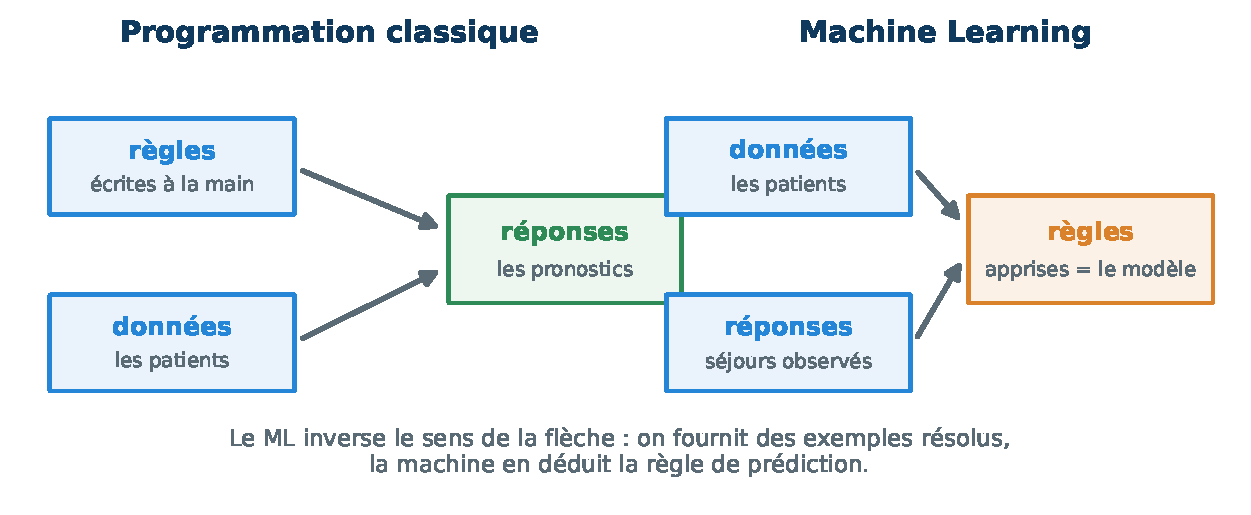
\includegraphics[width=0.78\linewidth]{f0_paradigm}
\vspace{-2pt}

{\scriptsize En programmation classique, les règles sont écrites à la main et appliquées aux données. En Machine Learning, on fournit des couples (données, réponses) et la machine \textbf{produit la règle} — qu'on appelle alors un \textbf{modèle}.}
\end{frame}

\begin{frame}{Qu'ont en commun tous ces exemples ?}
\begin{itemize}\small
  \item Dans chaque cas, la règle de décision est \textbf{trop complexe ou trop mouvante} pour être écrite à la main.
  \item Dans chaque cas, on dispose d'\textbf{exemples résolus} : des transferts étiquetés fraude/légitime, des patients dont le séjour est connu, des saisons dont le rendement est mesuré.
  \item Dans chaque cas, la machine \textbf{extrait la règle des exemples} — et l'applique aux cas futurs.
\end{itemize}
\begin{ucadret}[La transition]
{\small Trois ingrédients reviennent toujours : une \textbf{tâche}, de l'\textbf{expérience} (les exemples), et une mesure de \textbf{performance}. Il ne reste qu'à en faire une définition — c'est exactement ce que fit Tom Mitchell.}
\end{ucadret}
\end{frame}

% #####################################################################
\section{Définir le Machine Learning}

\begin{frame}{La définition historique — Samuel}
\begin{ucaddef}[Arthur Samuel — 1959]
{\small Le Machine Learning est «~le champ d'étude qui donne aux ordinateurs la capacité d'\textbf{apprendre sans être explicitement programmés}~». \emph{(« Field of study that gives computers the ability to learn without being explicitly programmed. »)}}
\end{ucaddef}
\begin{ucadex}[L'anecdote fondatrice]
{\small Samuel écrit un programme de \textbf{jeu de dames} qui joue des dizaines de milliers de parties \emph{contre lui-même}. À force de parties, le programme apprend quelles positions mènent à la victoire — et finit par \textbf{battre Samuel lui-même}, qui n'était pourtant pas un grand joueur. La machine a dépassé son programmeur : elle n'a pas été programmée pour bien jouer, elle a \emph{appris} à bien jouer.}
\end{ucadex}
\end{frame}

\begin{frame}{La définition moderne — Mitchell, formellement}
\begin{ucaddef}[L'idée en une phrase]
{\small La définition de Samuel dit \emph{quoi} ; celle de Tom Mitchell (1997) dit \emph{comment le vérifier} — elle rend l'apprentissage \textbf{mesurable}.}
\end{ucaddef}
\begin{ucadform}[Définition de Mitchell]
{\small Un programme \textbf{apprend} de l'expérience $E$, relativement à une tâche $T$ et une mesure de performance $P$, si sa performance sur $T$, mesurée par $P$, \textbf{s'améliore avec} $E$.}
\end{ucadform}
{\small Décryptage : $T$ est \emph{ce qu'on veut faire} ; $E$ est \emph{ce qu'on montre à la machine} (les exemples) ; $P$ est \emph{le chiffre qui dit si ça marche}. Apprendre $=$ voir $P$ monter quand $E$ grandit. Sans $P$, impossible de distinguer un programme qui apprend d'un programme qui récite.}
\end{frame}

\begin{frame}{Exemple — Mitchell instancié deux fois}
\begin{ucadex}[Sur la fraude mobile money]
{\small $T$ : classer chaque transfert en fraude ou légitime. \quad $E$ : l'historique de millions de transferts, \emph{étiquetés} après enquête. \quad $P$ : la proportion de fraudes correctement détectées sur les transferts du mois suivant.}
\end{ucadex}
\begin{ucadex}[Sur le fil rouge du cours]
{\small $T$ : prédire si le séjour hospitalier d'un patient sera long. \quad $E$ : un registre de $10\,000$ patients passés, pour lesquels la réponse est connue. \quad $P$ : la proportion de prédictions correctes sur des patients \emph{jamais vus}.}
\end{ucadex}
{\small Le triplet $(T, E, P)$ est la \textbf{grille de lecture} de tout problème de ML : chaque séance du cours commencera, implicitement, par le remplir.}
\end{frame}

\begin{frame}{Exercice — instancier Mitchell}
\begin{ucadrec}[Énoncé]
{\small Une coopérative veut prédire le \textbf{rendement d'arachide} (en tonnes par hectare) de chaque parcelle, à partir de la pluviométrie, du type de sol et de la date de semis. Elle dispose des relevés complets des $12$ dernières campagnes. Identifier $T$, $E$ et $P$.}
\end{ucadrec}
\pause
\begin{ucadex}[Correction]
{\small $T$ : prédire le rendement d'une parcelle (un \emph{nombre}). \quad $E$ : les relevés des $12$ campagnes — parcelles \emph{avec} leur rendement observé. \quad $P$ : l'écart moyen entre rendement prédit et rendement réel sur une campagne \emph{non utilisée} pour apprendre. Noter que $P$ n'est pas «~un pourcentage de bonnes réponses~» : la sortie étant un nombre, on mesure une \emph{erreur} — la distinction arrive dans quelques diapositives.}
\end{ucadex}
\end{frame}

% #####################################################################
\section{Situer le ML entre IA et Deep Learning}

\begin{frame}{Trois cercles emboîtés}
\centering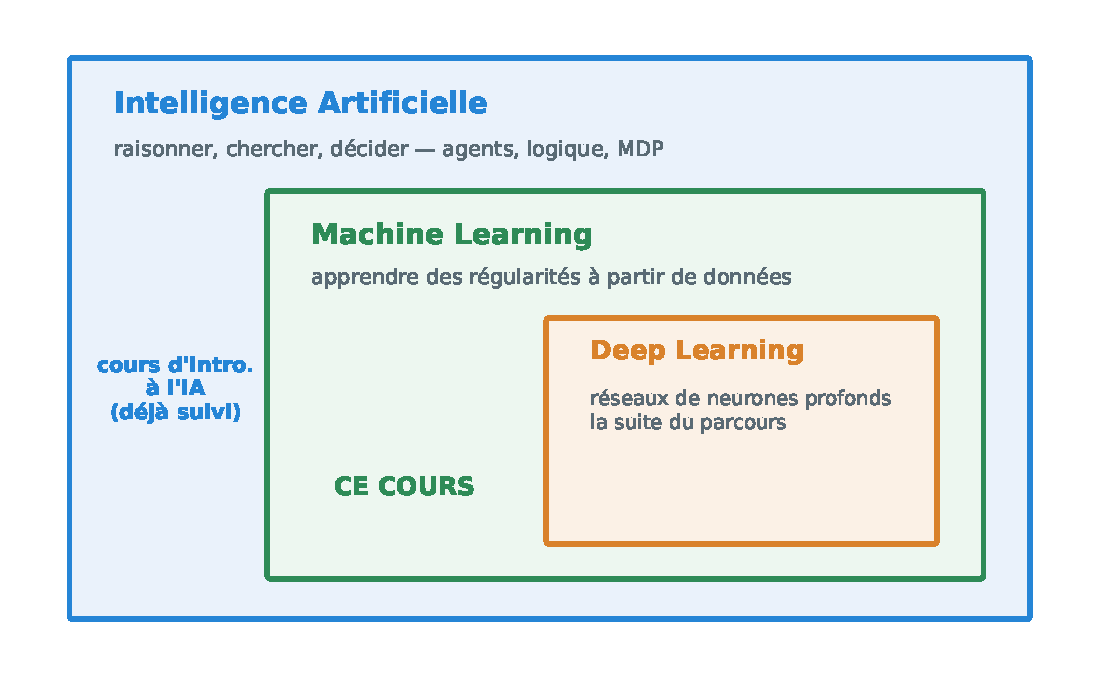
\includegraphics[width=0.62\linewidth]{f0_aimldl}
\vspace{-2pt}

{\scriptsize Le ML est un \textbf{sous-domaine} de l'Intelligence Artificielle ; le Deep Learning est un \textbf{sous-domaine} du ML. Ce cours occupe le cercle du milieu.}
\end{frame}

\begin{frame}{En amont et en aval de ce cours}
\begin{itemize}\small
  \item \textbf{En amont — l'IA symbolique} (cours d'Introduction à l'IA) : des agents qui \emph{raisonnent sur des règles données} — recherche de chemins, logique, décision sous incertitude. Les règles y sont \textbf{écrites}, pas apprises.
  \item \textbf{Ici — le Machine Learning} : la machine \emph{apprend les régularités} directement des données. C'est le changement de paradigme de la diapositive «~Programmer autrement~».
  \item \textbf{En aval — le Deep Learning} : du ML dont les modèles sont des \textbf{réseaux de neurones profonds}, rois des images, du son et du texte. Tout ce qui s'apprend ici (données, entraînement, généralisation, évaluation) y reste valable — ce cours pose les fondations.
\end{itemize}
\begin{ucadret}[Le pont avec le cours d'IA]
{\small Le raisonnement bayésien et les MDP rencontrés en IA reviendront : le ML en est le prolongement naturel, quand les probabilités cessent d'être données et doivent être \emph{estimées à partir des données}.}
\end{ucadret}
\end{frame}

% #####################################################################
\section{Les trois types d'apprentissage}

\begin{frame}{Trois manières d'apprendre}
\centering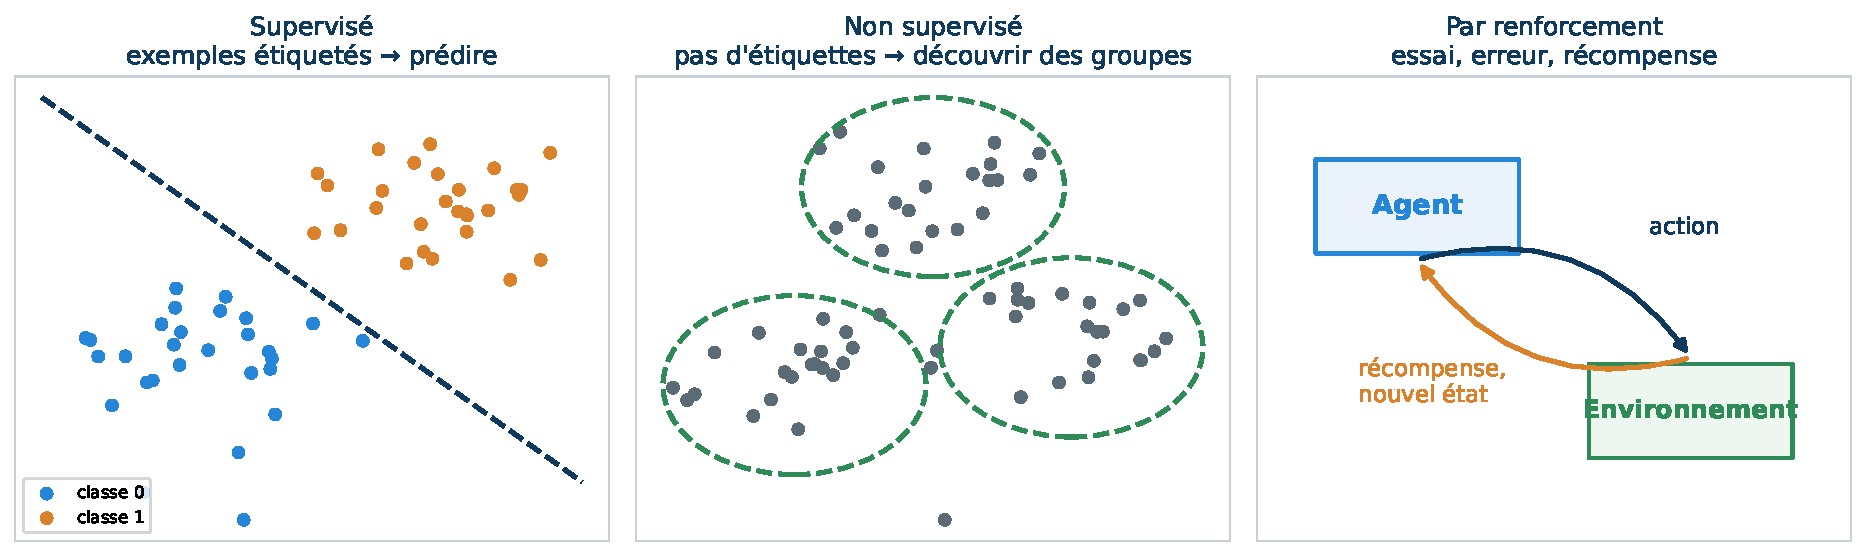
\includegraphics[width=0.97\linewidth]{f0_types}
\vspace{-2pt}

{\scriptsize \textbf{Supervisé} : des exemples \emph{étiquetés}, une frontière à apprendre. \textbf{Non supervisé} : des données \emph{sans} étiquettes, des structures à découvrir. \textbf{Par renforcement} : un agent qui apprend de ses \emph{récompenses}, par essai-erreur.}
\end{frame}

\begin{frame}{L'apprentissage supervisé}
\begin{ucaddef}[Définition]
{\small En apprentissage \textbf{supervisé}, chaque exemple est accompagné de la \textbf{bonne réponse} (l'étiquette). La machine apprend l'application entrée $\to$ sortie, pour répondre ensuite sur des entrées nouvelles.}
\end{ucaddef}
\begin{itemize}\small
  \item Si la sortie est un \textbf{nombre} (rendement, prix, durée), on parle de \textbf{régression}.
  \item Si la sortie est une \textbf{catégorie} (fraude/légitime, séjour long/court), on parle de \textbf{classification}.
\end{itemize}
{\small C'est de très loin le type le plus utilisé en pratique — l'essentiel de la valeur créée par le ML aujourd'hui repose sur ce simple schéma entrée $\to$ sortie. Les Séances 3 à 8 lui sont consacrées.}
\end{frame}

\begin{frame}{Exercice — régression ou classification ?}
\begin{ucadrec}[Énoncé]
{\small Pour chaque tâche, dire s'il s'agit de régression ou de classification : \textbf{(a)} prédire la durée d'un séjour hospitalier en jours ; \textbf{(b)} décider si un mail est un spam ; \textbf{(c)} prédire le prix d'un mouton de Tabaski ; \textbf{(d)} reconnaître la lettre manuscrite sur une copie ($26$ possibilités).}
\end{ucadrec}
\pause
\begin{ucadex}[Correction]
{\small \textbf{(a)} régression — la sortie est un nombre ; \textbf{(b)} classification — deux catégories ; \textbf{(c)} régression ; \textbf{(d)} classification — la sortie est une catégorie parmi $26$, pas une quantité qu'on mesure. Le critère est toujours la \emph{nature de la sortie}, jamais celle des entrées.}
\end{ucadex}
\end{frame}

\begin{frame}{L'apprentissage non supervisé}
\begin{ucaddef}[Définition]
{\small En apprentissage \textbf{non supervisé}, les données arrivent \textbf{sans étiquettes}. La machine ne prédit pas une réponse : elle \emph{découvre une structure} cachée dans les données.}
\end{ucaddef}
\begin{itemize}\small
  \item \textbf{Clustering} : regrouper les exemples qui se ressemblent — segmenter les clients du mobile money en profils d'usage, sans qu'aucun profil n'ait été défini à l'avance.
  \item \textbf{Réduction de dimension} : compresser des centaines de variables en quelques axes essentiels, pour visualiser ou accélérer.
\end{itemize}
{\small Plus exploratoire, souvent préparatoire au supervisé — la Séance 9 y revient.}
\end{frame}

\begin{frame}{L'apprentissage par renforcement}
\begin{ucaddef}[Définition]
{\small En apprentissage \textbf{par renforcement}, un \textbf{agent} agit dans un environnement et reçoit des \textbf{récompenses}. Personne ne lui montre la bonne action : il la découvre par \emph{essai-erreur}, en maximisant sa récompense cumulée.}
\end{ucaddef}
\begin{itemize}\small
  \item C'est le cadre des \textbf{MDP} rencontrés en Introduction à l'IA — avec une différence décisive : les probabilités de transition et les récompenses ne sont plus \emph{données}, l'agent doit les \emph{apprendre en agissant}.
  \item Le programme de dames de Samuel en est l'ancêtre : ses parties contre lui-même \emph{sont} l'essai-erreur.
\end{itemize}
\begin{ucadfront}[Pour être complet]
{\small Il existe des variantes intermédiaires (semi-supervisé, auto-supervisé) — hors du périmètre de ce cours, qui se concentre sur le supervisé et ouvre une porte vers le non supervisé.}
\end{ucadfront}
\end{frame}

\begin{frame}{Exercice — quel type d'apprentissage ?}
\begin{ucadrec}[Énoncé]
{\small Pour chaque situation, identifier le type d'apprentissage : \textbf{(a)} regrouper $50\,000$ abonnés télécom en profils de consommation, sans catégories prédéfinies ; \textbf{(b)} prédire si un patient sera réadmis sous $30$ jours, à partir de dossiers où la réadmission est connue ; \textbf{(c)} faire apprendre à un thermostat à climatiser une salle en le récompensant quand la température est bonne et la consommation basse.}
\end{ucadrec}
\pause
\begin{ucadex}[Correction]
{\small \textbf{(a)} non supervisé (clustering) — aucune étiquette ; \textbf{(b)} supervisé (classification) — l'étiquette réadmis/non réadmis est présente dans les données ; \textbf{(c)} par renforcement — pas d'étiquette, mais une récompense et de l'essai-erreur. La question à se poser est toujours : \emph{qu'est-ce que la machine reçoit pour apprendre ?}}
\end{ucadex}
\end{frame}

% #####################################################################
\section{Le vocabulaire et le but du jeu}

\begin{frame}{Les cinq mots du métier}
\begin{center}\small \renewcommand{\arraystretch}{1.3}
\begin{tabular}{p{3.1cm} p{4.5cm} p{4.2cm}}
\textbf{Terme} & \textbf{Ce que c'est} & \textbf{Dans le fil rouge}\\\hline
\textbf{Caractéristiques} (\emph{features}, $X$) & les variables qui décrivent un exemple & âge, glycémie, hémoglobine, fièvre, saison\\
\textbf{Étiquette} (\emph{label}, $y$) & la réponse à prédire & séjour long ou court\\
\textbf{Exemple} & un cas complet — caractéristiques et étiquette & un patient du registre\\
\textbf{Jeu d'entraînement} & les exemples montrés à la machine & les patients passés\\
\textbf{Modèle} & la règle apprise qui prédit $y$ à partir de $X$ & le produit final du cours\\
\end{tabular}\end{center}
\end{frame}

\begin{frame}{Le but du jeu : généraliser}
\begin{ucaddef}[Définition]
{\small \textbf{Généraliser}, c'est prédire juste sur des exemples \textbf{jamais vus} pendant l'apprentissage. C'est le \emph{seul} objectif du ML : un modèle qui ne sait répondre que sur ses données d'entraînement n'a rien appris — il a mémorisé.}
\end{ucaddef}
\begin{ucadfront}[Analogie]
{\small Un étudiant qui récite par cœur les exercices du TD peut échouer à l'examen : réussir le TD ne prouve rien, réussir des exercices \emph{nouveaux} prouve la compréhension. Pour le modèle, c'est pareil — on gardera toujours des données de côté pour lui faire passer un \textbf{examen}.}
\end{ucadfront}
{\small Cette idée — séparer des données pour évaluer honnêtement — structure tout le cours ; elle est mise en pratique dès la Séance 3.}
\end{frame}

\begin{frame}{Ce que le ML ne fait pas}
\begin{itemize}\small
  \item \textbf{Pas de miracle sur de mauvaises données} : un modèle nourri de données fausses ou biaisées apprend des règles fausses ou biaisées — \emph{garbage in, garbage out}.
  \item \textbf{Pas de généralisation au-delà de son expérience} : un modèle entraîné sur les patients d'une seule région peut se tromper lourdement sur le reste du pays — l'échantillon doit représenter la cible.
  \item \textbf{Pas de causalité} : le ML capture des \emph{régularités}, pas des causes — corrélation n'est pas causalité.
  \item \textbf{Pas de magie} : un modèle ne remplace ni la compréhension du problème, ni la connaissance du terrain — il les \emph{outille}.
\end{itemize}
\begin{ucadpiege}[Erreur fréquente]
{\small Croire un chiffre de performance sans demander \emph{sur quelles données} il a été mesuré. Un score calculé sur les données d'entraînement est une illusion — toute la suite du cours apprend à mesurer honnêtement.}
\end{ucadpiege}
\end{frame}

\begin{frame}{La route des dix séances}
\centering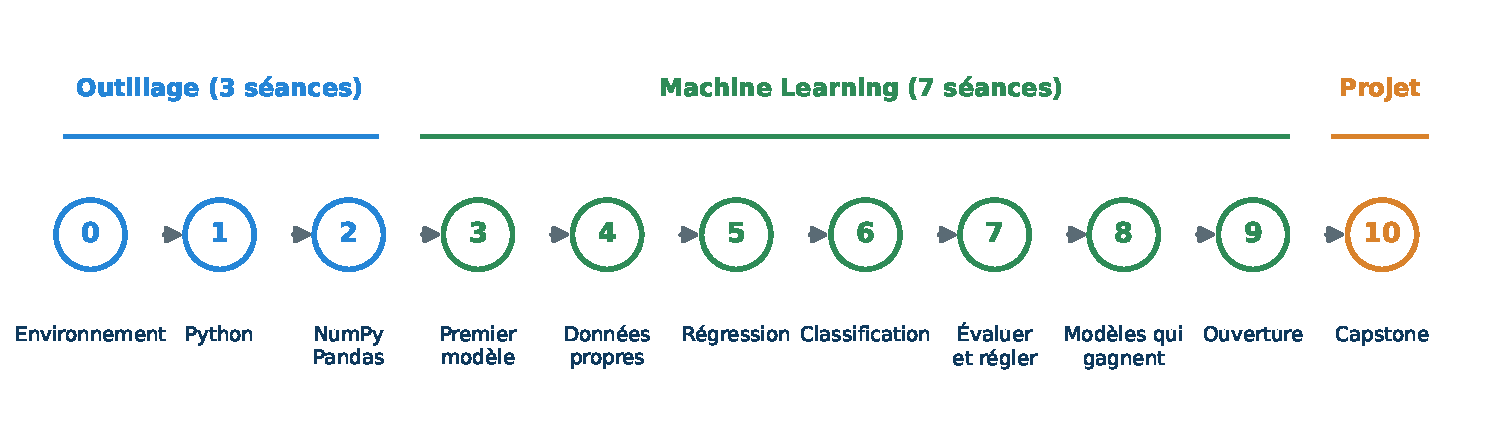
\includegraphics[width=0.99\linewidth]{f0_route}
\vspace{-2pt}

{\scriptsize Trois séances d'outillage (environnement, Python, données), sept séances de Machine Learning — presque toutes consacrées au \textbf{supervisé}, avec l'ouverture non supervisée en Séance 9 — et un projet final sur données réelles. Tout commence ici, par l'atelier.}
\end{frame}

\begin{frame}{Les données du cours}
\begin{ucaddef}[Le fil rouge]
{\small \textbf{DataSANTÉ-221} : un registre hospitalier de $10\,000$ patients de cinq régions du Sénégal — âge, glycémie, hémoglobine, fièvre, saison — avec la durée de séjour observée. Toutes les notions du cours s'y incarnent d'abord.}
\end{ucaddef}
\begin{itemize}\small
  \item Le fil rouge donne un \textbf{terrain familier} : à chaque nouvelle notion, les données sont déjà connues.
  \item S'y ajoutent des \textbf{jeux réels} : Pima (diabète), California Housing (immobilier), Heart Disease — et, pour le capstone, des données de compétitions \textbf{Zindi}, ancrées dans le contexte africain.
\end{itemize}
\end{frame}

% #####################################################################
\section{La pile logicielle}

\begin{frame}{Pourquoi un environnement local}
\begin{ucaddef}[Le choix du cours]
{\small Le cours travaille \textbf{en local} : tout s'installe sur la machine de chacun. C'est l'outillage du métier — celui qui fonctionne sans connexion, sur ses propres fichiers, et que l'on contrôle de bout en bout.}
\end{ucaddef}
\begin{itemize}\small
  \item \textbf{Autonomie} : pas de dépendance à une connexion stable ni à un service distant.
  \item \textbf{Réalisme} : en entreprise comme en recherche, on travaille dans un environnement maîtrisé.
  \item \textbf{Pérennité} : l'installation d'aujourd'hui servira aux cours et projets des années suivantes.
\end{itemize}
\begin{ucadpiege}[Erreur fréquente]
{\small Compter sur un service en ligne « le jour J » : une coupure de connexion pendant une évaluation ou une démonstration, et plus rien ne tourne. L'atelier local, lui, ne dépend que de la machine.}
\end{ucadpiege}
\end{frame}

\begin{frame}{La pile : qui s'appuie sur qui}
\begin{columns}[c]
\column{0.46\textwidth}
\begin{ucaddef}[Quatre étages]
{\small \textbf{Anaconda} installe Python et l'outil \texttt{conda} ; \texttt{conda} crée l'\textbf{environnement} \texttt{ml} ; l'environnement contient les \textbf{bibliothèques} ; \textbf{Jupyter} est la salle de travail où on les utilise.}
\end{ucaddef}
{\small Toute la séance consiste à monter ces étages, un par un, dans l'ordre.}
\column{0.5\textwidth}
\centering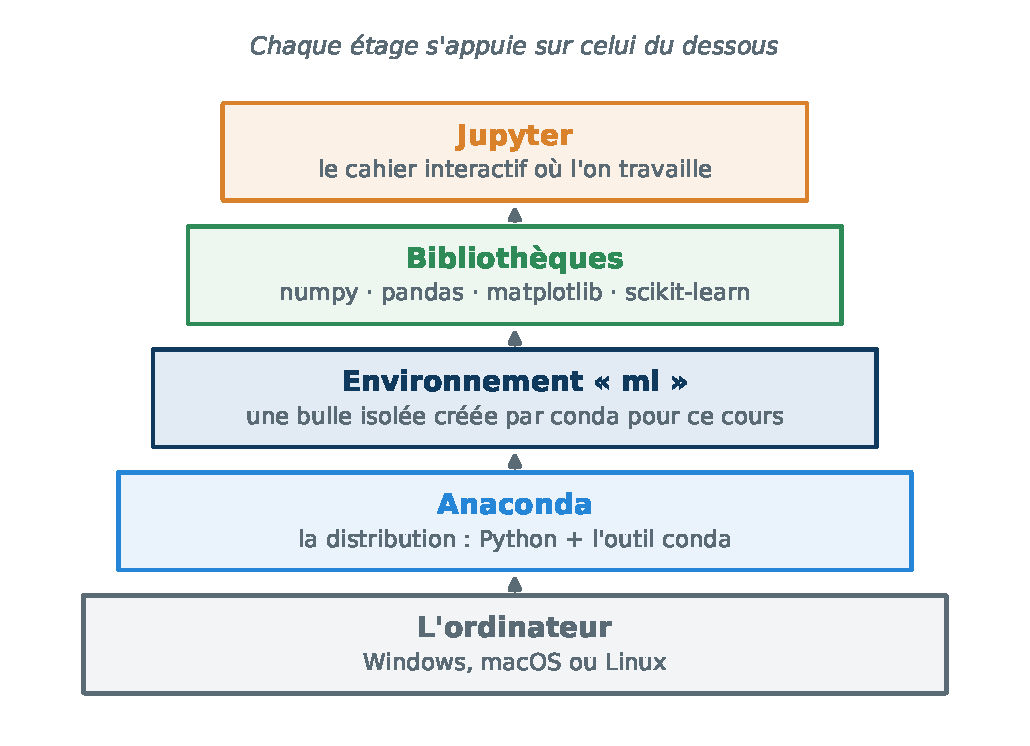
\includegraphics[width=0.92\linewidth]{f0_stack}
\end{columns}
\end{frame}

\begin{frame}{Le vocabulaire de l'atelier}
\begin{center}\small \renewcommand{\arraystretch}{1.3}
\begin{tabular}{p{3.0cm} p{8.6cm}}
\textbf{Terme} & \textbf{Ce que c'est}\\\hline
\textbf{Terminal} & La fenêtre où l'on tape des commandes texte (Anaconda Prompt sous Windows ; Terminal sous macOS et Linux).\\
\textbf{Distribution} & Un paquet « tout-en-un » : Anaconda fournit Python, \texttt{conda} et des centaines de bibliothèques.\\
\textbf{Environnement} & Une bulle isolée contenant une version de Python et ses bibliothèques. Le nôtre s'appelle \texttt{ml}.\\
\textbf{Bibliothèque} & Du code prêt à l'emploi qu'on importe : \texttt{numpy}, \texttt{pandas}, \texttt{matplotlib}, \texttt{scikit-learn}.\\
\textbf{Notebook} & Un document interactif mêlant texte, code et résultats — le format de tous les TP.\\
\end{tabular}\end{center}
\end{frame}

\begin{frame}{Les quatre bibliothèques du cours}
\begin{itemize}\small
  \item \textbf{NumPy} — le calcul sur tableaux de nombres : rapide, vectorisé, à la base de tout le reste.
  \item \textbf{Pandas} — les tableaux de données étiquetés (lignes, colonnes nommées) : lire un fichier, filtrer, agréger.
  \item \textbf{Matplotlib} — les graphiques : voir ses données avant de les modéliser.
  \item \textbf{scikit-learn} — les modèles de Machine Learning, tous derrière la même interface \texttt{fit} / \texttt{predict}.
\end{itemize}
{\small Les Séances 1 et 2 apprennent à manier les trois premières ; \texttt{scikit-learn} entre en scène à la Séance 3 — et n'en sort plus.}
\end{frame}

\begin{frame}{Jupyter : le cahier de laboratoire}
\centering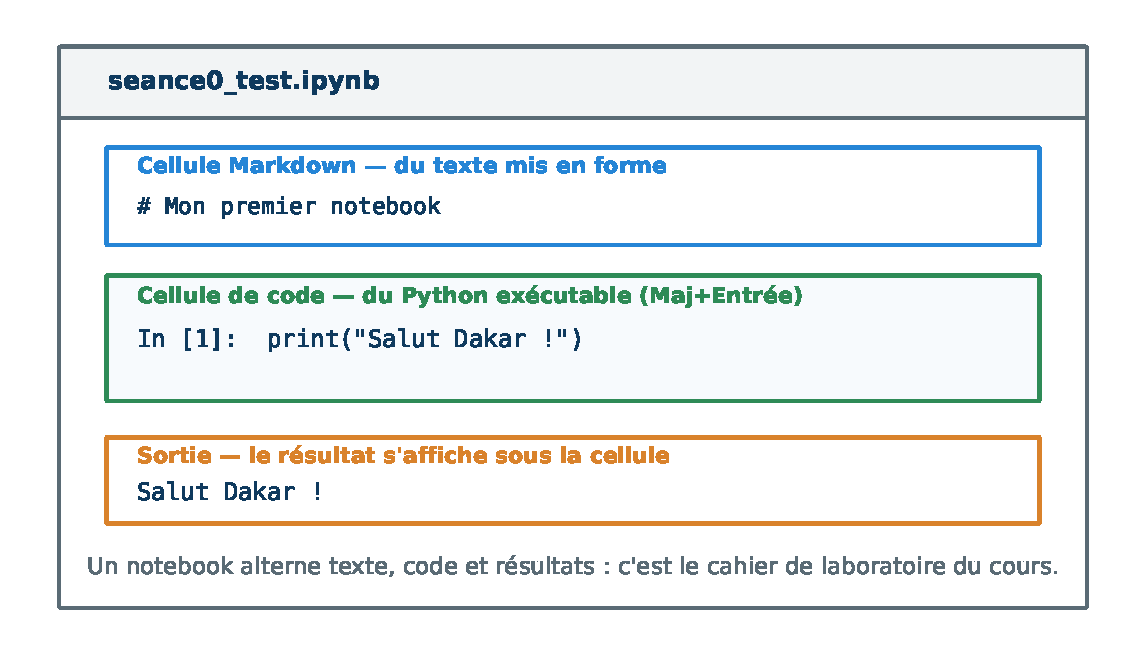
\includegraphics[width=0.62\linewidth]{f0_notebook}
\vspace{-2pt}

{\scriptsize Un notebook est une suite de \textbf{cellules}. Les cellules \emph{Markdown} portent le texte ; les cellules de \emph{code} s'exécutent avec \textbf{Maj+Entrée} et affichent leur résultat juste en dessous. On expérimente, on corrige, on réexécute — le cycle naturel du ML.}
\end{frame}

\begin{frame}{Exercice — qui fait quoi ?}
\begin{ucadrec}[Énoncé]
{\small Associer chaque besoin à l'outil de la pile : \textbf{(a)} créer une bulle isolée pour le cours ; \textbf{(b)} lire un fichier de patients et filtrer les plus de $60$ ans ; \textbf{(c)} entraîner un arbre de décision ; \textbf{(d)} écrire et exécuter le TP cellule par cellule.}
\end{ucadrec}
\pause
\begin{ucadex}[Correction]
{\small \textbf{(a)} \texttt{conda} (commande \texttt{conda env create}) ; \textbf{(b)} \texttt{pandas} ; \textbf{(c)} \texttt{scikit-learn} ; \textbf{(d)} Jupyter. Chaque outil a un rôle unique — c'est leur empilement qui fait l'atelier.}
\end{ucadex}
\end{frame}

% #####################################################################
\section{Installation pas à pas}

\begin{frame}{La feuille de route en six étapes}
\begin{ucadret}[Le chemin complet]
{\small \textbf{1.} Télécharger Anaconda. \;\textbf{2.} L'installer. \;\textbf{3.} Vérifier \texttt{conda} dans un terminal. \;\textbf{4.} Créer l'environnement \texttt{ml}. \;\textbf{5.} L'activer. \;\textbf{6.} Lancer Jupyter et exécuter la cellule de vérification.}
\end{ucadret}
{\small Chaque étape se vérifie avant de passer à la suivante : une installation qui échoue à l'étape $4$ se répare à l'étape $4$ — jamais en recommençant tout.}
\end{frame}

\begin{frame}{Étape 1 — télécharger Anaconda}
\begin{itemize}\small
  \item Se rendre sur \textbf{anaconda.com/download} et choisir l'installeur de son système.
  \item \textbf{Windows} : installeur graphique \texttt{.exe} ($64$ bits). \quad \textbf{macOS} : installeur \texttt{.pkg} — attention au choix entre puce \emph{Apple Silicon} (M1 à M4) et \emph{Intel}. \quad \textbf{Linux} : script \texttt{.sh}.
  \item Le fichier pèse environ $1$ Go : prévoir le téléchargement \emph{avant} la séance si la connexion est lente — il sera aussi distribué sur clé USB en début de séance.
\end{itemize}
\begin{ucadpiege}[Erreur fréquente]
{\small Sur macOS, télécharger la version Intel sur une machine Apple Silicon (ou l'inverse) : l'installation passe, mais les performances s'effondrent. Vérifier sa puce dans «~À propos de ce Mac~».}
\end{ucadpiege}
\end{frame}

\begin{frame}{Étape 2 — installer}
\begin{itemize}\small
  \item \textbf{Windows} : lancer l'\texttt{.exe}, accepter les choix par défaut — installation «~Just Me~», \emph{ne pas} cocher l'ajout manuel au \texttt{PATH} (l'\emph{Anaconda Prompt} s'en charge proprement).
  \item \textbf{macOS} : ouvrir le \texttt{.pkg} et suivre l'assistant.
  \item \textbf{Linux} : \texttt{bash Anaconda3-*.sh}, accepter la licence, accepter l'initialisation de \texttt{conda} en fin d'installation, puis rouvrir le terminal.
\end{itemize}
\begin{ucadpiege}[Erreur fréquente]
{\small Installer dans un dossier dont le chemin contient des \textbf{espaces ou des accents} («~\texttt{C:\textbackslash Users\textbackslash Mamadou Bâ\textbackslash...}~») : certains outils s'y perdent. En cas de doute, choisir un chemin court et sans accents, par exemple \texttt{C:\textbackslash anaconda3}.}
\end{ucadpiege}
\end{frame}

\begin{frame}[fragile]{Étape 3 — ouvrir le terminal et vérifier}
{\small \textbf{Windows} : menu Démarrer $\to$ \emph{Anaconda Prompt}. \quad \textbf{macOS / Linux} : application \emph{Terminal}.}
\begin{lstlisting}[style=sh]
conda --version
# conda 24.x.y     <- la version exacte importe peu : elle doit s'afficher
\end{lstlisting}
{\small Si une version s'affiche, l'étage Anaconda est posé. Sinon, voir le dépannage en fin de séance — la cause est presque toujours l'utilisation du mauvais terminal sous Windows.}
\begin{ucadret}[Réflexe à prendre]
{\small Sous Windows, \emph{toutes} les commandes du cours se tapent dans l'\textbf{Anaconda Prompt} — jamais dans l'invite de commandes classique, qui ne connaît pas \texttt{conda}.}
\end{ucadret}
\end{frame}

\begin{frame}[fragile]{Le fichier de l'environnement}
{\small L'environnement du cours est décrit dans un petit fichier texte, \texttt{environnement-ml.yml}, distribué avec la séance :}
\begin{lstlisting}[style=sh]
name: ml
channels:
  - defaults
dependencies:
  - python=3.11
  - numpy
  - pandas
  - matplotlib
  - scikit-learn
  - jupyter
  - flake8
\end{lstlisting}
{\small Une ligne par bibliothèque : le fichier \emph{est} la liste de courses de l'atelier. Le même fichier recrée le même environnement sur n'importe quelle machine — c'est sa force.}
\end{frame}

\begin{frame}[fragile]{Étape 4 — créer l'environnement ml}
{\small Dans le terminal, se placer dans le dossier contenant le fichier (commande \texttt{cd}), puis :}
\begin{lstlisting}[style=sh]
conda env create -f environnement-ml.yml
# Telechargement et installation des paquets : quelques minutes...
\end{lstlisting}
{\small En cas d'absence du fichier, la commande équivalente tient en une ligne :}
\begin{lstlisting}[style=sh]
conda create -n ml python=3.11 numpy pandas matplotlib scikit-learn jupyter flake8
\end{lstlisting}
{\small La création ne se fait qu'\textbf{une seule fois} : l'environnement reste installé pour tout le cours.}
\end{frame}

\begin{frame}[fragile]{Étape 5 — activer l'environnement}
\begin{lstlisting}[style=sh]
conda activate ml
# l'invite change :   (ml) C:\Users\fatou>
\end{lstlisting}
\begin{ucaddef}[Ce que fait l'activation]
{\small Activer, c'est \textbf{entrer dans la bulle} : à partir de là, \texttt{python} et \texttt{jupyter} désignent ceux de l'environnement \texttt{ml}, avec ses bibliothèques. Le préfixe \texttt{(ml)} dans l'invite confirme qu'on est dedans.}
\end{ucaddef}
\begin{ucadret}[Réflexe à prendre]
{\small \textbf{À chaque nouvelle session de travail} : ouvrir le terminal, taper \texttt{conda activate ml}, \emph{puis} lancer Jupyter. L'activation ne survit pas à la fermeture du terminal.}
\end{ucadret}
\end{frame}

\begin{frame}[fragile]{Étape 6 — lancer Jupyter}
\begin{lstlisting}[style=sh]
(ml) jupyter notebook
# Le navigateur s'ouvre sur http://localhost:8888 ...
\end{lstlisting}
\begin{itemize}\small
  \item Le navigateur affiche les fichiers du dossier courant ; \textbf{New} $\to$ \textbf{Python 3} crée un notebook.
  \item Le terminal devient le \textbf{moteur} de Jupyter : il affiche des messages tant que Jupyter tourne.
  \item Pour arrêter proprement : fermer les notebooks, puis \texttt{Ctrl+C} dans le terminal.
\end{itemize}
\begin{ucadpiege}[Erreur fréquente]
{\small Fermer la fenêtre du terminal pendant le travail : Jupyter s'éteint avec elle et les cellules cessent de répondre. Le terminal reste ouvert, en arrière-plan, toute la session.}
\end{ucadpiege}
\end{frame}

\begin{frame}[fragile]{Le premier notebook}
{\small Créer un notebook, le renommer \texttt{seance0\_test}, puis taper dans la première cellule :}
\begin{lstlisting}
print("Salut Dakar !")
\end{lstlisting}
{\small \textbf{Maj+Entrée} exécute la cellule : le texte s'affiche dessous, et une cellule vide apparaît. C'est le geste fondamental — il sera répété des centaines de fois dans ce cours.}
\begin{ucadex}[Ce qui vient de se passer]
{\small La cellule a traversé toute la pile : Jupyter a transmis le code au Python de l'environnement \texttt{ml}, qui l'a exécuté et renvoyé le résultat. Quatre étages, un aller-retour — en quelques millisecondes.}
\end{ucadex}
\end{frame}

\begin{frame}[fragile]{La cellule de vérification}
{\small Dans une nouvelle cellule, vérifier que les quatre bibliothèques répondent :}
\begin{lstlisting}
import numpy, pandas, matplotlib, sklearn
print("numpy        :", numpy.__version__)
print("pandas       :", pandas.__version__)
print("matplotlib   :", matplotlib.__version__)
print("scikit-learn :", sklearn.__version__)
\end{lstlisting}
{\small Quatre numéros de version s'affichent : l'atelier est complet. Cette cellule est le \textbf{certificat d'installation} — elle ouvre tous les notebooks du cours, et son échec désigne immédiatement l'étage en panne.}
\end{frame}

\begin{frame}{Exercice — lire une commande}
\begin{ucadrec}[Énoncé]
{\small Un étudiant tape les trois commandes suivantes, dans cet ordre : \texttt{conda activate ml}, puis \texttt{jupyter notebook}, puis il ferme le terminal. \textbf{(a)} Que fait chacune des deux commandes ? \textbf{(b)} Que se passe-t-il à la fermeture du terminal ?}
\end{ucadrec}
\pause
\begin{ucadex}[Correction]
{\small \textbf{(a)} La première \emph{entre dans la bulle} \texttt{ml} (le préfixe \texttt{(ml)} apparaît) ; la seconde démarre Jupyter, dont le terminal devient le moteur. \textbf{(b)} Le moteur s'éteint avec le terminal : le notebook ouvert dans le navigateur ne répond plus. Il fallait laisser le terminal ouvert.}
\end{ucadex}
\end{frame}

\begin{frame}{Et l'éditeur du métier : VS Code}
\begin{ucadfront}[Pour aller plus loin]
{\small \textbf{Visual Studio Code} (code.visualstudio.com) est l'éditeur le plus répandu du métier. Avec ses extensions \emph{Python} et \emph{Jupyter}, il ouvre les notebooks du cours et sait utiliser l'environnement \texttt{ml} (sélecteur de noyau, en haut à droite).}
\end{ucadfront}
\begin{itemize}\small
  \item Son installation est \textbf{recommandée mais pas exigée} : Jupyter dans le navigateur suffit pour tout le cours.
  \item Son vrai intérêt viendra avec les projets : fichiers \texttt{.py}, recherche dans le code, \texttt{flake8} intégré.
\end{itemize}
\end{frame}

\begin{frame}{Organiser ses fichiers}
\begin{ucadret}[Une arborescence pour tout le cours]
{\small Créer un dossier \texttt{intro-ml} (chemin \textbf{sans espaces ni accents}), avec un sous-dossier par séance : \texttt{seance00}, \texttt{seance01}, \dots{} Chaque sous-dossier reçoit le notebook de TP et les données de la séance. Lancer Jupyter \emph{depuis} \texttt{intro-ml}.}
\end{ucadret}
{\small Une arborescence stable évite la moitié des pannes : fichiers de données « introuvables », notebooks égarés, doublons. L'autre moitié se traite à la section suivante.}
\end{frame}

% #####################################################################
\section{Dépannage}

\begin{frame}{Symptôme et remède}
\begin{center}\small \renewcommand{\arraystretch}{1.3}
\begin{tabular}{p{5.4cm} p{6.6cm}}
\textbf{Symptôme} & \textbf{Cause probable et remède}\\\hline
\texttt{conda~:~commande introuvable} & Mauvais terminal (Windows) : ouvrir l'\emph{Anaconda Prompt}. Sous Linux : rouvrir le terminal après l'installation.\\
\texttt{ModuleNotFoundError~:~sklearn} & Jupyter lancé \emph{hors} de la bulle : fermer, \texttt{conda activate ml}, relancer.\\
L'invite n'affiche pas \texttt{(ml)} & L'activation a été oubliée ou faite dans un autre terminal.\\
Les cellules ne répondent plus & Le terminal-moteur a été fermé : relancer Jupyter (l'environnement, lui, est intact).\\
\texttt{EnvironmentLocationNotFound} & L'environnement n'a jamais été créé : refaire l'étape $4$.\\
\end{tabular}\end{center}
\end{frame}

\begin{frame}{Exercice — diagnostiquer une panne}
\begin{ucadrec}[Énoncé]
{\small Une étudiante lance \texttt{jupyter notebook}, ouvre un notebook et exécute \texttt{import sklearn} : \texttt{ModuleNotFoundError}. Pourtant, l'étape $4$ s'était terminée sans erreur la veille. \textbf{(a)} Quelle est la cause la plus probable ? \textbf{(b)} Donner la séquence exacte de commandes qui répare.}
\end{ucadrec}
\pause
\begin{ucadex}[Correction]
{\small \textbf{(a)} Jupyter a été lancé \emph{hors} de l'environnement \texttt{ml} : il utilise le Python de base, où \texttt{scikit-learn} n'est pas installé. L'environnement, créé la veille, existe toujours — il n'était simplement pas \emph{activé}. \textbf{(b)} Fermer Jupyter (\texttt{Ctrl+C}), puis : \texttt{conda activate ml} et \texttt{jupyter notebook}.}
\end{ucadex}
\end{frame}

\begin{frame}{La checklist de sortie}
\begin{ucadret}[Avant de quitter la séance]
{\small \textbf{1.} \texttt{conda --version} répond. \;\textbf{2.} \texttt{conda activate ml} affiche le préfixe \texttt{(ml)}. \;\textbf{3.} Jupyter s'ouvre dans le navigateur. \;\textbf{4.} La cellule de vérification affiche les quatre versions. \;\textbf{5.} Le dossier \texttt{intro-ml} existe, sans espaces ni accents dans son chemin.}
\end{ucadret}
{\small Cinq cases cochées : la machine est prête pour les dix séances. Une case manquante : la table « symptôme et remède » donne la réparation — et la séance ne se termine pas avant que tout le monde coche les cinq.}
\end{frame}

% #####################################################################
\section{Synthèse}

\begin{frame}{À retenir — Séance 0}
\begin{ucadret}[L'essentiel]
\begin{itemize}\small
  \item Le ML \textbf{inverse la programmation} : on fournit des exemples résolus, la machine produit la règle — le modèle.
  \item \textbf{Mitchell} rend l'apprentissage mesurable : une tâche $T$, une expérience $E$, une performance $P$ qui s'améliore.
  \item \textbf{IA $\supset$ ML $\supset$ DL} — et trois types d'apprentissage : supervisé (étiquettes), non supervisé (structures), par renforcement (récompenses).
  \item Le but unique : \textbf{généraliser} — prédire juste sur du jamais-vu, pas réciter l'entraînement.
  \item L'atelier : Anaconda $\to$ \texttt{conda} $\to$ environnement \texttt{ml} $\to$ bibliothèques $\to$ Jupyter ; le rituel de chaque session est \texttt{conda activate ml} puis \texttt{jupyter notebook}.
\end{itemize}
\end{ucadret}
\end{frame}

\begin{frame}{Pièges fréquents}
\begin{itemize}\small
  \item Confondre régression et classification : le critère est la \emph{nature de la sortie} (nombre ou catégorie).
  \item Croire qu'un modèle « comprend » : il capture des régularités — corrélation n'est pas causalité.
  \item Évaluer un modèle sur ses données d'entraînement : mémoriser n'est pas généraliser.
  \item Travailler hors de l'environnement \texttt{ml} : tout semble marcher — jusqu'au premier \texttt{import sklearn}.
  \item Fermer le terminal qui fait tourner Jupyter : les cellules cessent de répondre.
\end{itemize}
\end{frame}

\begin{frame}{Prochaine séance}
\begin{ucadfront}[Séance 1 — Python de zéro]
{\small L'atelier est monté ; il reste à apprendre la langue qu'on y parle. La Séance 1 enseigne Python en partant de zéro — variables, listes, conditions, boucles, fonctions — entièrement dans Jupyter, sur l'environnement installé aujourd'hui.}
\end{ucadfront}
\end{frame}

\begin{frame}{Références}
\begin{itemize}\small
  \item T. M. Mitchell, \emph{Machine Learning}, McGraw-Hill, 1997.
  \item A. Géron, \emph{Hands-On Machine Learning with Scikit-Learn, Keras \& TensorFlow}, 3\textsuperscript{e} éd., O'Reilly, 2022.
  \item A. C. Müller, S. Guido, \emph{Introduction to Machine Learning with Python}, O'Reilly, 2016.
  \item G. James, D. Witten, T. Hastie, R. Tibshirani, \emph{An Introduction to Statistical Learning}, 2\textsuperscript{e} éd., Springer, 2021.
  \item Documentation officielle : conda (docs.conda.io) ; Jupyter (docs.jupyter.org).
\end{itemize}
\end{frame}

\end{document}
